\documentclass[twoside]{protokoll}
\usepackage{graphicx}
\usepackage{tabularx} % for better table formatting
\usepackage{booktabs} % for better table formatting
\usepackage{float} 
\praktikum{I}
\usepackage{subfig}
\usepackage{amsmath}

\versuchsgebiet{(E-Lehre)}


\teilnehmer{Maximilian Carlos Menke, 434170}
\teilnehmer{Andrea Roth, 428396}
\gruppe{A3}

\begin{document}
 
\section{1E3 Gekoppelte LC-Schwingkreise}

\begin{aufgabe}{Grundlagen}
  Knappe Beschreibung der theoretischen Grundlagen, Angabe der
  benötigten Formel(n), ohne Herleitung. Definition der verwendeten
  Formelzeichen.
\end{aufgabe}
\section{Gurndlagen}
Ein einfacher Schwingkreis besteht aus einer in Reihe geschlateten Spule und einem Kondensator.
Angenommen der Kondensator ist am anfang aufgeladen (1),
dann entlädt sich der Kondensator(2), der durch die Spule fließende Strom induziert ein Magnetfeld (3), und das Magnetfeld induziert einen Gegenstrom sodass der Kondensator entgegengesetzt aufgeladen wird.
Anschließend passiert das ganze umgekehrt sodass man wieder im anfangszustand ist.
Dadurch entsteht eine Schwingung.
Dieser Schaltplan ist allerdings idealisiert, da die elektrischen Wiederstände der Bauteile nicht berücksichtigt wurden.
Aufgrund der Kettenregen (die Summe aller Spannungen muss 0 sein), ergibt sich die DGL:
\begin{equation}
    \frac{d^2 Q}{dt^2} + \frac{R}{L} \cdot \frac{d U}{dt} + \frac{1}{LC} \cdot U = 0
\end{equation}
Aus der DGL kann man folgende beziehungen ableiten. $\omega_0$ ist dabei die Eigenfrequenz ohne dämpfung, $\omega$ die Eigenfrequenz mit dämpfung.
$\delta$ ist die Dämpfungskonstante.
\begin{equation}
    \delta = \frac{R}{2L}
\end{equation}
\begin{equation}
    \Rightarrow R = 2 L \cdot \delta
\end{equation}
\begin{equation}
    \omega_0 = \frac{1}{\sqrt{L \cdot C}}
\end{equation}
\begin{equation}
    \omega = \sqrt{\omega_0^2 - \delta^2}
\end{equation}
Dabei sieht die allgemeine Schwingungsgleichung wie folgt aus:
\begin{equation}
    U(t) = U_0 \cdot e ^ {-\delta t} + U_{off}
\end{equation}

Man kann zwei Schwingkreise aber auch koppeln, da mit einer Spule eine Spannung in der Spule des anderen Schwingkreises induziert werden kann.
Dafür müssen die Schwingkreise in ca die gleiche Eigenfrequenz haben, was bei uns der Fall ist, da sie baugleich sind.
Wenn zwei Schwingkreise gekoppelt sind, und nur in einem Schwingkreis eine Schwingung erzwungen wird, kommt es anschließend zu Schwebung.
Die Fundamentalschwingungen sind dabei die Schwingungen welche man in diesem Falle im Fourierspektrum als Maxima erkennen kann.
Dabei ist $f_-$ das rechte Maximum und $f_+$ das linke.
Dabei gilt für die Fundamentalschwingungen:
\begin{equation}
    \omega_+ = \frac{\omega_0}{\sqrt{1 + k}}
\end{equation}
\begin{equation}
    \omega_- = \frac{\omega_0}{\sqrt{1 - k}}
\end{equation}
\begin{equation}
    \Rightarrow k = \frac{\omega_0^2}{\omega_+^2} - 1 = - \frac{\omega_0^2}{\omega_-^2} + 1
\end{equation}
\begin{equation}
    \Rightarrow k = \frac{f_-^2 - f_+^2}{f_-^2 + f_+^2}
\end{equation}
Im Falle der Schwebung kann man beim verlauf der Spannung am Kondensator sehen, das es eine innere Schwingung und eine Einüllende gibt. \\
Dabei gilt für die innere Frequenzen $f_k$ und die Schwebungsfrequenz $f_{schw}$:
\begin{equation}
    f_k = \frac{f_- + f_+}{2}
\end{equation}
\begin{equation}
    f_{schw} = \frac{f_- - f_+}{2}
\end{equation}
    

Wenn beide Schwingkreise angeregt werden, dann kann man zwischen gleichsinniger und gegensinniger Aufladung unterscheiden.
Bei gleichsinniger Aufladung fließen die Ströme in die gleiche Richtung durch die Spulen.
Hier kann man im Fourierspektrum $f_-$ als Maximum messen.
Bei gegensinniger Aufladung kann man $f_+$ als Maximum des Fourierspektrums messen.

So kann man sowohl mit der Schwebung, wie auch mit gleich und gegensinniger Anregung den Kopplungsgrad mithilfe der oben angegeben Formel bestimmen.:

Zudem kann man aufgrund der Dämpfung von dem internen Wiederstand unseres Schwingkreises eine leichte zeitliche Verschiebung zwischen Maximaler Spannung am einen Kondensator und Nulldurchgang der Spannung am anderen Kondensator.
Diese ist für $ k < 0.2$ (was bei uns der Fall sein wird):
\begin{equation}
    \Delta t \approx \frac{2 \pi}{f_{schw}} \left[ \frac{1}{\pi} - \arctan{\left( \frac{k}{R} \cdot \sqrt{\frac{L}{C}} \right)} \right]
\end{equation}


 
\begin{aufgabe}{Versuchsaufbau und Versuchsdurchführung}
  Beschreibung des Versuchsaufbaus einschließlich
  Schaltbild. Beschreibung der Versuchsdurchführung: verwendete
  Messwerterfassungseinstellungen, Messbereiche, Triggerbedingungen,
  etc.
\end{aufgabe}

\subsection{Kurze Zusammenfassung des Aufbaus und Durchführung}

Detaillierter Aufbau und Durchführung zu den einzelnen Versuchsteilen, finden Sie am Anfang von den jeweiligen Abschnitten. 
Hier soll der Gesamtversuch kurz Dargestellt werden.\\

Der Versuch besteht aus insgesamt 3 Teilen. Für den ersten Teilversuch haben wir zwei LC-Schwingkreise Aufgebaut mit gleichen Bauteilen und die Schwingung in diesen einzeln gemessen. 
Diese sind Schwingkreise mit je einem Kondensator und einer Spule.
Als Widerstand in der Schaltung liegt nur der Innenwiederstand von Spule und Kondensator und den Kabeln vor. 
An den Schwingkreis wird eine Spannungsquelle angeschlossen, welche mithilfe eines Tasters kurzgeschlossen werden kann und den Schwingkreis schließt. 
Der Spannungsverlauf wird über dem Kondensator parallel gemessen. 
Dieser Teilversuch dient dazu den Einzelschwingkreis zu charakterisieren, dies wird Später benötigt zur Auswertung der gekoppelten Schwingkreise.\\

Zur Kopplung der Schwingkreise werden die Spulen nebeneinander gestellt und auch die Spannung am zweiten Kondensator gemessen. Durch drücken des Tasters wird eine Messung gestartet.
Als Einflussfaktoren auf den Kopplungsgrad wird das Variieren des Abstands der Spulen untersucht und der Einfluss eines Eisenkerns\\

Im letzten Teilversuch werden nun beide Kondensatoren mit der gleichen Spannungsquelle geladen. 
So, dass der Strom ein mal gleich sinnig durch die Spulen läuft und ein mal gegen sinnig. Die Schwingungen haben wir wieder an beiden Kondensatoren gemessen, und daraus die Frequenzen $f_+$ und $f_-$ bestimmt. 
 

\begin{aufgabe}{Vorversuch: Charakterisierung der verwendeten Bauteile}
  Charakterisieren Sie die verwendeten Bauteile mit Digitalvoltmeter
  bzw. Messbrücke.
\end{aufgabe}

Vor der Durchführung der Versuche, und zum späteren Vergleich der Messungen mit unseren Erwartungen haben wir die Bauteile charakterisiert. Dies haben wir mit einer Messbrücke getan. 

\begin{figure}[H]
    \centering
    \includegraphics[width=0.8\textwidth]{bilder/Messbrücke_10Ohm.pdf}
    \caption{Charakterisierung des 10 $\mu F$ Kondensator}
\end{figure}

In dem Bild zu sehen ist die Messbrücke, an die Stelle wo der Kondensator ist, wir das Bauteil angeschlossen. Das Bild ist noch mit unserem ersten Kondensator, diesen haben wir im Verlauf des Experiments gegen einen kleineren ausgetauscht, und alle Messungen mit dem kleineren wiederholt.\\

Die Messungen mit der Messbrücke haben einen statistischen Messfehler von 0.25\%.\\
Für die Messung haben wir unseren Frequenzbereich von 1kHz eingestellt.
 (In dem Bild auf 100Hz weil wir da noch den 10 $\mu F$ messen, und wir mit diesem geringere Frequenzen hatten.) 
 Die Spulle haben wir ebenfalls gemessen wenn diese einen Eisenkern hatten, um den Einfluss von diesem auf Widerstand und Induktivität zu bestimmen.
So konnten wie sämtliche Bauteile Charakterisieren und sind für unseren zweiten Aufbau (mit kleinerem Kondensator) zu folgenden Ergebnissen gekommen:\\
    
\begin{table}[H]
        \centering
        \begin{tabularx}{1.0\textwidth}{X l} % adjust width as needed
            \toprule
            \textbf{Bauteil} & \textbf{Messung} \\
            \midrule
            Spule 1 & R = (2.344 $\pm$ 0.006) $\Omega$ \quad L = (9.02 $\pm$ 0.02)mH \\
            mit Eisenkern & R = (2.700 $\pm$ 0.007) $\Omega$ \quad L = (55.79 $\pm$ 0.14)mH \\
            \midrule
            Spule 2 & R = (2.423 $\pm$ 0.006) $\Omega$ \quad L = (8.98 $\pm$ 0.02)mH \\
            mit Eisenkern & R = (2.650 $\pm$ 0.007) $\Omega$ \quad L = (56.10 $\pm$ 0.14) mH \\
            \midrule
            Kondensator 1 & (2.301 $\pm$ 0.006) $\mu$F \\
            Kondensator 2 & (2.262 $\pm$ 0.006) $\mu$F \\
            \bottomrule
        \end{tabularx}
        \caption{Ergebnisse der Messung mit dem Multimeter}
        \label{tab:mytable}
    \end{table}

\begin{aufgabe}{Ungekoppelte Schwingung}
  Zeigen Sie den Verlauf der Kondensatorspannungen für den
  ungekoppelten Fall und bestimmen Sie die Schwingungsfrequenz samt
  Messunsicherheit. Vergleichen Sie sie mit Ihrer Erwartung.
\end{aufgabe}

\subsection{Ungekoppelter Schwingkreis}

\subsubsection{Materialien}


Vor Beginn des Versuchs haben wir unsere Bauteile gewählt. Wir hatten uns erst für einen $10\mu F$ Kondensator entschieden und eine Spule mit 500 Windungen.
Dies erachteten wir als Sinnvoll da wir wissen, dass $ f \propto \frac{1}{LC}$ gilt. 

So haben wir eine niedrigere Frequenz als bei kleineren Kondensatoren. 
Diese Spule haben wir gewählt, da eine Spule mit weniger Windungen zwar geringeren Widerstand hat aber auch eine geringere Kopplung. Eine Spule mit mehr Windungen würde zwar die Kopplung vergrößern, jedoch auch den Widerstand. \\

Bei den gekoppelten Schwingkreisen, stellten wir jedoch fest, dass bereits ab einem Abstand von 1cm keine Kopplung mehr vorlag. 
Aufgrund dessen haben wir dann unseren $10\mu F$ Kondensator durch einen $2.2 \mu F$ ausgetauscht. \\


Zuerst haben zwei ungekoppelte Schwingkreise aufgebaut mit gleichen Bauteilen.
 
\textbf{Material Liste}
\begin{itemize}
  \item 2x Spule $9mH$
  \item 2x Kondensator $2.2 \mu F$
  \item Spannungsqelle vom Cassy
  \item Schalter
  \item Kabel
  \item Steckplatte DIN A4
\end{itemize}

\subsubsection{Aufbau}

Der erste Schwingkreis wurde dabei wie unten skizziert aufgebaut.
Darauf zu achten ist, dass die Spannung parallel am Kondensator zu messen ist, mit dem Sensor CASSY. Der Schalter Schließt die Spannungsquelle kurz, und schließt somit den Schwingkreis.
\begin{figure}[H]
    \centering
    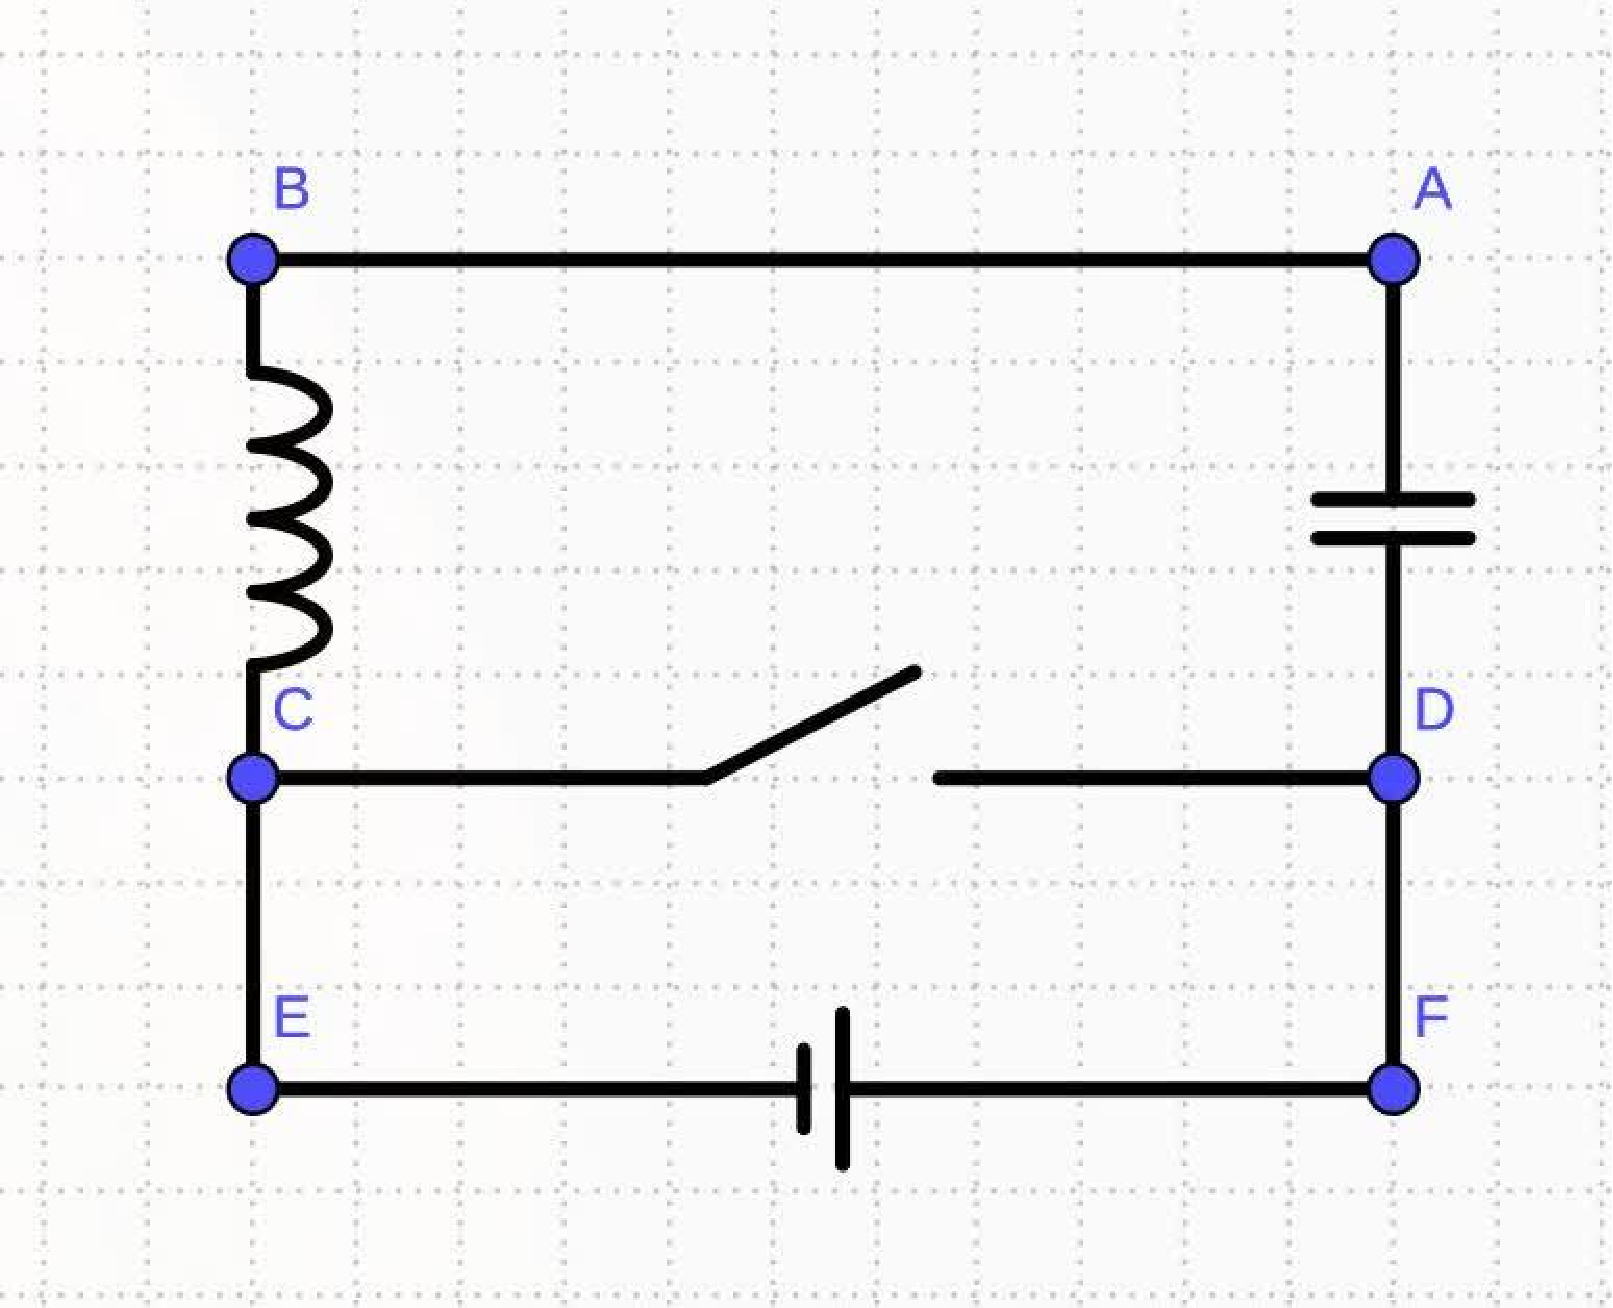
\includegraphics[width=0.8\textwidth]{schaltplan-einzelschwingkreis.pdf}
    \caption{Aufbau der Schwingkreise}
\end{figure}
\begin{figure}[H]
    \centering
    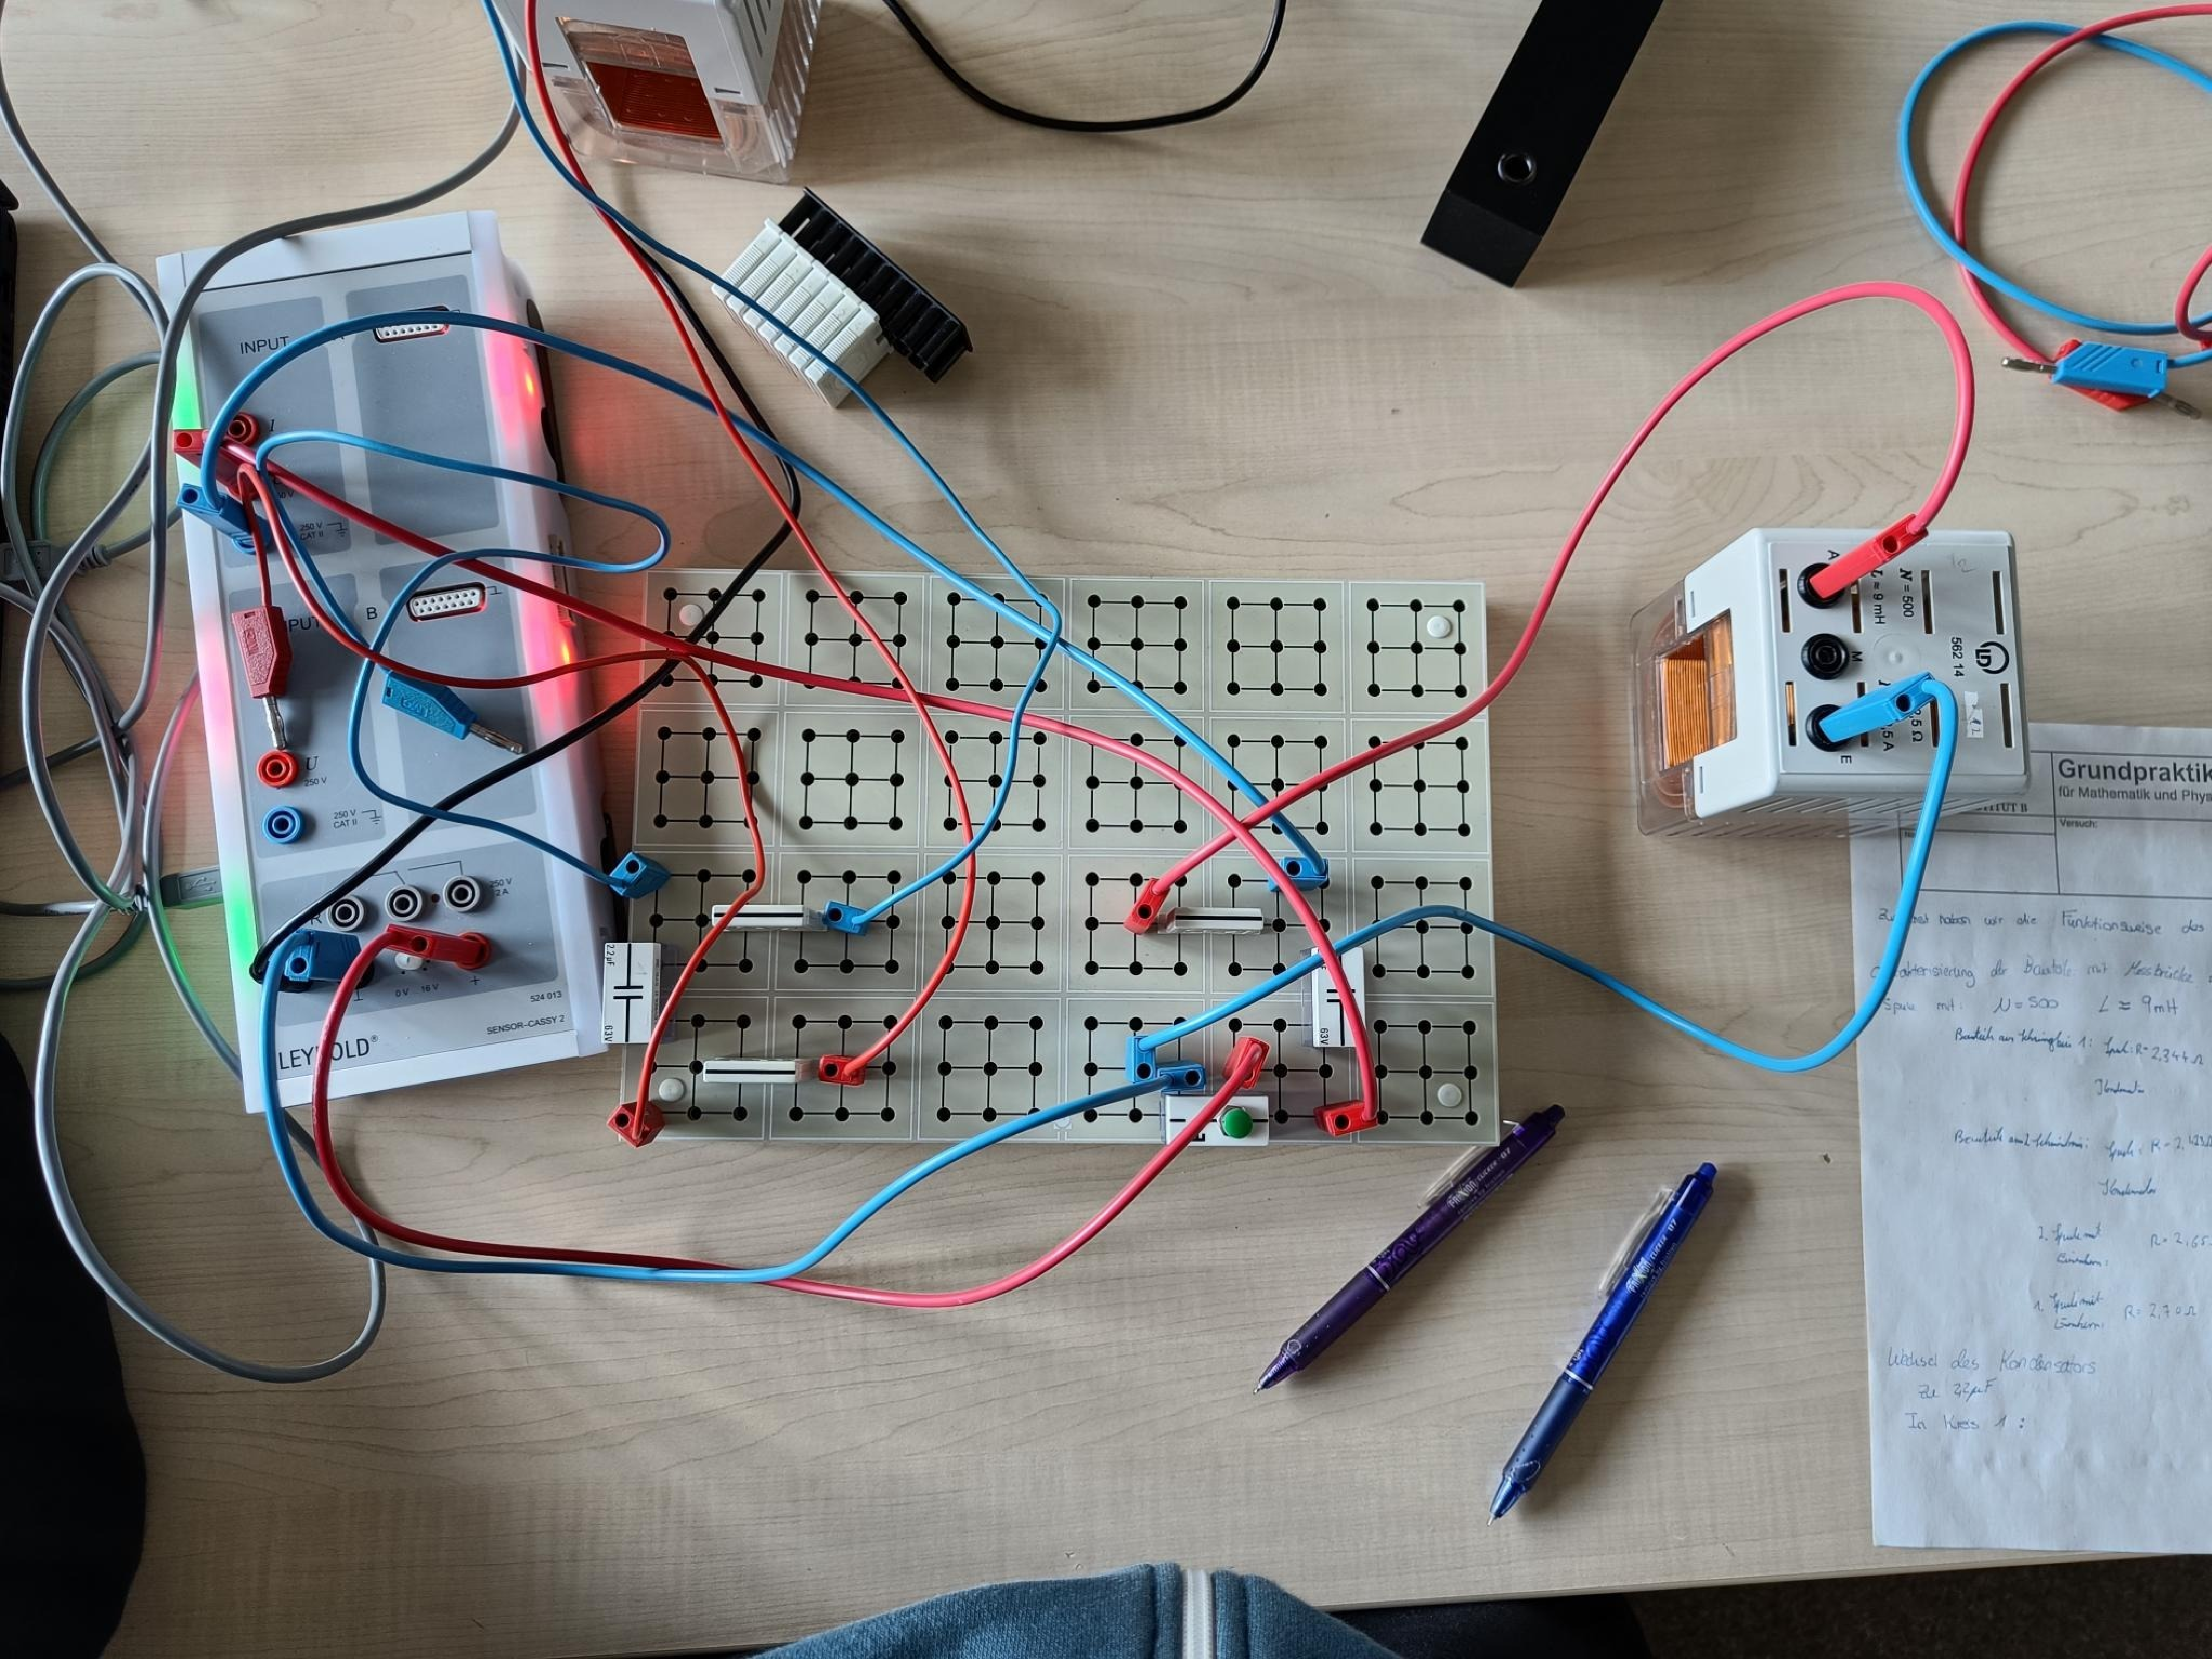
\includegraphics[width=0.8\textwidth]{bilder/schwingkreis2.pdf}
    \caption{Aufbau der beiden Schwingkreise}
\end{figure}

Oben ist ein Bild von beiden Schwingkreisen zu sehen, wobei links der 1. ist und rechts der 2.
Hier wird der 2. Schwingkreis vermessen, weshalb der 1. Schwingkreis auch nicht eingesteckt machen im CASSY.
 
Zudem haben wir mit Spule zwei und Kondensator zwei einen zweiten Schwingkreis aufgebaut.
Der Aufbau und die Schaltskizze des zweiten Schwingkreises ist gleich zu dem des ersten.
Insgesamt hatten wir 2 getrennte Schwingkreise, aber nur einen Schalter und eine Spannungsquelle (da wir die Schwingkreise später koppeln werden).
Deshalb haben wir die Spannungsquelle und den Schalter dann jeweils umgesteckt, um die zwei Schwingkreise getrennt zu messen.




\subsubsection{Durchführung}
Zuerst haben wir eine Spannung von $U_0 = 6.2V$ angelegt da bei dieser Spannung die Maximale Stromstärke der Spule ( $2.5A$ ) nicht überschritten wird.
Also haben wir als Spannungsbereich des CASSY-10V bis 10V eingestellt.
Anschließend haben wir ein paar Testmessungen gemacht, um die optimalen Messeinstellungen zu finden.
Diese Testmessungen haben wir jedoch noch mit unserer 'alten' Kapazität gemacht ( $C = 10 \mu F$ ).
Beim einbauen der neuen haben wir die Messparameter aber angepasst.\\
Dafür haben wir die Periodendauer ohne Widerstand genähert (da dieser für eine grobe Abschätzung vernachlässigbar klein ist).
\begin{equation}
    T = 2 \pi \sqrt{LC} = 2 \pi \sqrt{9mH \cdot 2.2 \mu F} = 884 \mu s
\end{equation}
Nach dem Nequisst Theorem muss die Abtastrate mindestens doppelt so groß sein wie die Frequenz.
Um eine ausreichende Auflösung des Fourier Peaks zu haben, und da diese Messung nur eine Abschätzung war, haben wir $ 50 \mu s $ als Messintervall gewählt, da dieses mehr als das 10x ist.

 
Die Schwingung im Schwingkreis startet in dem Moment, in dem man den Taster drückt, und sich der Kondensator anfängt zu entladen, da soll auch die Messung starten.
Damit der Schwingkreis ungestört schwingen kann, muss der Taster auch während der gesamten Messung gedrückt bleiben.
Entsprechend haben wir den Trigger vom Cassy auf 6.1V fallende Flanke gestellt um die Messung zu starten.
Dabei haben wir 6.1V gewählt, da so noch der Großteil der ersten Schwingungsperiode mit aufgezeichnet wird.
0.1V Abstand sind genug um Störeffekte vom schließen des Schalters nicht auf zu zeichnen.
Den zweiten Schwingkreis haben wir dabei 10 mal vermessen, um die Statistische Unsicherheit auf die Frequenz zu bestimmen.

Den ersten Schwingkreis haben wir dabei nur einmal vermessen, da wir davon ausgehen können, das die Statistische Unsicherheit bei beiden Schwingkreisen gleich ist, da wir den gleichen Aufbau verwendet haben und auch sonst gleiche Messbedingungen hatten.



Nachdem die Messung beendet ist, wir das Frequenz Spektrum mit hilfe einer Fouriertransformation analysiert.
Die Länge der Messung beeinflusst dabei die Auflösung der Fouriertransformation.
 
\begin{figure}[H]
    \centering
    \includegraphics[width=0.8\textwidth]{plots/schwingkreis-alt-test-200us-0.01s_fft_zoom.pdf}
    \caption{Zoomin Plot der FFT der Testmessung mit Messdauer = 0.01s}
\end{figure}
Wie zu sehen ist bei diese Testmessung, ist das Fourierspektrum nur auf $ \pm 100Hz $ genau. Das bedeutet das die Messdauer von 0.01s zu kurz ist.
Als Messdauer haben wir später 0.5s Sekunden gewählt, da wir dann einen zufridenstellenden (weniger als 0.1\%) Abeshe Fehler hatten.

Hier eine übersicht der Messeinstellungen. Dabei haben wir den Kanal auf den getriggert wird immer auf den gestellt, an welchem der zu messende Schwingkreis angeschlossen war.
\begin{table}[H]
    \centering
    \begin{tabularx}{1\textwidth}{X X X X} % adjust width as needed
        \toprule
        \textbf{Intervall} & \textbf{Messzeit} & \textbf{Trigger} & \textbf{Messbereich (für beide Eingäge)} \\
        \midrule
        200$\mu$s  & 0.5s & 6.1V fallend & -10V - 10V \\
        \bottomrule
    \end{tabularx}
    \caption{Messwertserfassungseinstellungen des CASSY}
    \label{tab:mytable}
\end{table}
     
Anschließend haben wir noch zwei Rauschmessung gemacht: einmal mit geöffnetem und einmal mit geschlossenem Schalter nach dem Schwingvorgang.
Diese haben wir gemacht, um daraus Offsets zu berechnen um unsere Messung des Wiederstandes zu präzisieren.


\subsubsection{Rohdaten}

Insgesamt hatten wir also die Kondenstorspannung beim Schwingungsvorgang in zweiten Schwingkreis 10x gemessen. Und im ersten Schwingkreis ein mal. 
So wie eine Rauschmessung bei 0V und bei ca. 6V. 

\begin{figure}[H]
    \centering
    \includegraphics[width=1\textwidth]{plots/schwingkreis_2_01.pdf}
    \caption{Schwingungsverlauf im zweiten Schwingkreis}
\end{figure}

Oben können sie Exemplarisch einen Schwingungsverlauf im zweiten Schwingkreis sehen. 
Das obere Bild zeigt die Messung über die gesamte Messdauer. 
Sehr gut kann hier der Exponentielle Abfall der Amplitude erkannt werden. Bereits nach ca. 0.03s ist die Amplitude auf null abgefallen. 
Das Messen des großen Zeitintervalls ergibt sin, dass dies die Auflösung bei der FFT erhöht.
\begin{figure}[H]
    \centering
    \includegraphics[width=1\textwidth]{plots/schwingkreis_1_01.pdf}
    \caption{Schwingungsverlauf im ersten Schwingkreis}
\end{figure}
hier noch der Schwingungsverläufe von unserem Ersten Schwingkreis. Dieser sieht Augenscheinlich sehr ähnlich zu den des zweiten aus.
Dies ist auch zu erwarten, da wir gleich Bauteil verwendet haben.

Das die zwei Schwingungen sehr ähnlich sind, kann man sehr gut daran erkennen, wenn man in den noch schwingenden Bereich der Messung zoomt.
\begin{figure}[H]
    \centering
    \includegraphics[width=1\textwidth]{plots/schwingkreise_zoom.pdf}
    \caption{Schwingungsverlauf der beiden Schwingkreis zoom-in}
\end{figure}
Hier können wir sehen, dass die Schingungen dem gleichen Kosinus Förmigen Verlauf folgen, Außerdem kann man hier bereits erkennen, dass Schwingkreis 2 eine höhere Frequenz hat.
Da die Bauteile nicht vollkommen identisch sein werden, ist dies nicht überraschend.\\
Die Amplituden fallen nach Augenmaß Exponentiell ab.

Zu diesen Schwingungsverläufen haben wir, jeweils eine FFT gemacht, um zu überprüfen, ob die Frequenz des Schwingkreis aus der Messung gut bestimmbar ist.
Oben ist der des zweiten Schwingkreis unten der des Ersten.


\begin{figure}[H]
    \centering
    \includegraphics[width=1\textwidth]{plots/schwingkreis_2_01_fft_complete.pdf}
    \caption{Schwingungsverlauf im ersten Schwingkreis}
\end{figure}

\begin{figure}[H]
    \centering
    \includegraphics[width=1\textwidth]{plots/schwingkreis_1_01_fft_complete.pdf}
    \caption{Schwingungsverlauf im ersten Schwingkreis}
\end{figure}

Zu sehen ist, dass wir einen klaren peak bei einer bestimmten Frequenz haben, es sind keine Frequenzen von anderen Schwingungen zu sehen. 
Dies war aus den Kosinus förmigen Verlauf der Messung zu erwarten. In diesem Zoom lässt sich jedoch noch keine Aussage über die genaue Frequenz der Schwingkreise treffen.

%TODO : Einfügen des Plots für die Nahaufnahme des FFT mit beiden Schwingkreisen

Im diesem Graphen ist ein Zoom-in der FFT zu sehen bei beiden Schwingungen, hier kann man gut erkennen, dass wir eine klare Spitze haben.Des weiteren kann man sehen, dass der Peak bei den beiden Schwingkreisen leicht gegeneinander verschoben sind 
Die Frequenz des Schwingkreis kann später durch weiteres zoomen festgestellt werden.


\subsubsection{Auswertung}
Da wir die Frequenz der Schwingkreise bestimmen sollten, haben wir uns die FFT im Bereich des Peaks genauer angesehen.
Zum bestimmen des Maximums haben wir immer den x-Wert genommen, welcher die größte Amplitude hat.
Alternativ hätten wir auch den Peakschwerpunkt nehmen können. Da die Verteilung aber unsymetrisch ist, haben wir uns dagegen entschieden.
\begin{figure}[H]
    \centering
    \includegraphics[width=1\textwidth]{plots/schwingkreis_1_01_fft_zoom.pdf}
    \caption{FFT Zoom vom ersten Schwinkgreis mit eingezeichnetem Peak}
    \label{fig:peak}
\end{figure}
Dabei kann dem zoom-in plot entnommen werden, das wir Messpunkte in 2Hz schritten haben.
Daraus ergibt sich für den Fehler auf Grund der Ablesegenauigkeit $ \frac{2Hz}{\sqrt{12}} = 0.6Hz $ 
 Diesen Ablesefehler nehmen wir als statistisch an.


Unten die Ergebnisse der einzelnen Messungen:


\begin{table}[H]
    \centering
    \begin{tabularx}{1\textwidth}{X X X X} % adjust width as needed
        \toprule
        \textbf{Messung} & \textbf{Schwingkreis} & \textbf{Frequenz} \\
        \midrule
        1 & 1 & 1106 Hz \\
        \midrule
        1 & 2 & 1118 Hz \\
        2 & 2 & 1116 Hz \\
        3 & 2 & 1118 Hz \\
        4 & 2 & 1118 Hz \\
        5 & 2 & 1116 Hz \\
        6 & 2 & 1118 Hz \\
        7 & 2 & 1116 Hz \\
        8 & 2 & 1118 Hz \\
        9 & 2 & 1118 Hz \\
        10& 2 & 1118 Hz \\
        \bottomrule
    \end{tabularx}
    \caption{Frequenzen von Schwingkreis 1 und 2}
\end{table}

Der Erwartungswert des 2. Schwingkreises ist:
\begin{equation}
    f_2 = 1117.3 Hz
\end{equation}
Dabei ist der Statistische Fehler auf den Einzelwert also die Frequenz, also die Unsicherheit auf den Erwartungswert, gegeben durch:
\begin{equation}
    \sigma_{f_2 stat} = 1.0 Hz
\end{equation}
Hier ist noch an zu merken, dass der Ablesefehler größer ist wenn wir die Auswertung mit Python machen, jedoch ist der statistische Fehler ( $\sigma_{f_{2stat}}$) größer als der Fehler aufgrund des Ablesens, weswegen wir hier keine Genauigkeit gewinnen, wenn wir die Auswertungsmethode gewinnen.

Somit ergibt sich der Fehler insgesamt aus der quadratischen Addition der beiden Fehlerbeiträge. Für den Fehler auf $f$ erhlaten wir.
\begin{equation}
\sigma_f = 1.2Hz
\end{equation}

%TODO frage nach ob man die frequenz mit dem maximum bestimmen kann.
\begin{figure}[H]
    \centering
    \includegraphics[width=1\textwidth]{plots/f_peak_errorbar.pdf}
    \caption{Schwingungsverlauf vom zweiten Schwingkreis zoom-in}
\end{figure}
Wie im Residueplot gut zu sehen ist, schwankt der Peak zwischen 2 Frequenzen.
 
Der Grund dafür ist in dem untenstehenden Plot gut zu erkennen.
\begin{figure}[H]
    \centering
    \includegraphics[width=1\textwidth]{plots/schwingkreis_2_02_fft_zoom.pdf}
    \caption{FFT Zoom von Schwingkreis 2 der 2. Messung}
    \label{fig:peak}
\end{figure}
Hier sieht man, wie bei der 2. Messung die Amplituden der Frequenz 1116Hz und 1118Hz sehr ähnlich sind.
Der Grund das die gefundene Amplitude um 2 Hz schwankt, liegt also in der Auflösung der FFT.
Da wir aber eine Messreihe von 10 Messungen durchgeführt haben, ist es aber nicht schlimm, das wir immer die Frequenz mit der Maximalen Amplitude genommen haben und nicht das Maximum abgeschätzt haben,
da wir durch das errechnen des Mittelwertes die Messungen entsprechend gewichten und mitteln. \\

Unsere theoretische überlegung bezüglich der erwarteten Frequenz, haben wir mithilfe folgender Formel gemacht:
\begin{equation}
    f_1 = \sqrt{\omega_0^2 - \delta^2} = \sqrt{ \frac{1}{LC} - \left( \frac{R}{2L} \right)^2}
\end{equation}
Da die erste Spule laut Messbrücke einen Wiederstand von $ 2.344  \Omega$ hat und die zweite von $2.423 \Omega$, und wir den Wiederstand des restlichen Stromkreises auf $0.3 \Omega$ geschätzt haben, schätzen wir einen Gesamtwiederstand von $ 2.644 \Omega$ für den ersten und $ 2.723 \Omega$ für den 2. Schwingkreis.
Mit den in der Messbrücke gemessen Werten für die Induktivität und Kapazität, haben wir folgende Frequenzen ausgerechnet und erwartet:
\begin{equation}
    f_1 = 1104.6 Hz
\end{equation}
\begin{equation}
    f_2 = 1116.4 Hz
\end{equation}
Damit liegen unsere Erwartungen innerhalb des statistischen Messfehlers von einem Hz. \\

Als nächstes haben wir die Rauschmessung ausgewertet. Hier eine Darstellung der Rauschmessung bei nicht gedrücktem Schalter als Histogramm:
\begin{figure}[H]
    \centering
    \includegraphics[width=1\textwidth]{plots/rauschen_0V_01.pdf}
    \caption{Rauschmessung bei 0V}
\end{figure}
Beim auswerten der Daten, haben wir für den Erwartungswert $ U_{off} = 4.882 mV$ erhalten, mit einer Standardabweichung von $\sigma_{off} = 0.761 mV$.
Dabei ist der Erwartungswert der Offset welchen wir später für die berechnung des Wiederstandes brauchen, und sigma die Statistische Unsicherheit auf die Messwerte.
Hierbei gehen wir davon aus, das beide Schwingkreise den gleichen Offset haben.

Als letztes haben wir, um den Wiederstand der beiden Schwingkreise zu bestimmen, die Einhüllende der beiden Schwingkreise bestimmt.
Dafür haben wir von den Spannungswerten der Messdaten den durch die Rauschmessung bestimmten Offset abgezogen.
Die Anpassung wurde mithilfe der Praktikums Libary durchgeführt.
 
Hier die Graphische Darstellung der Einhüllenden.
Die untere Einhüllende ist dabei die obere mal minus 1.
Diese haben wir noch zusätzlich dargestellt um die Genauigkeit der Anpassung besser zu beurteilen.
Für den Fit wurde das gesamte Messintervall verwendet, in dem Plot haben wir lediglich den Anfang dargestellt, da man dort die abweichung der Messwerte vom Fit besser beurteilen kann.
Als statistische Unsicherheit auf die Spannungsmesswerte haben dabei den Fehler von der Rauschmessung und den digitalisierungs Fehler genommen.
Den digitalisieruns Fehler haben wir mit der Formel $ \sigma_{digital} = \frac{V_{max} - V_{min}}{2^{12} \sqrt{12}}$ bestimmt.
Diesen nehmen wir als statistischen Fehler an, da wir davon ausgehen können das die Messwerte gleichverteilt im Intervall sind.
\begin{equation}
    \sigma_{U Stat} = \sqrt{ \sigma_{digital}^2 +  \sigma_{off}^2} = 2mV
\end{equation}
\begin{figure}[H]
    \centering
    \includegraphics[width=1\textwidth]{plots/schwingkreis_einhüllende_1.pdf}
    \caption{Einhüllende des ersten Schwingkreises}
\end{figure}
 
%TODO systematischer Fehler beachten
%TODO digitalisierungs fehler beachten
Gleiches haben wir beim 2. Schwingkreis gemacht.
Der Wiederstand konnte wie in den Grundlagen diskutiert, bestimmt werden mit $ U(t) = A \cdot e^{-t \cdot B} - U_{off}$:
Für den ersten Schwingkreis haben wir folgende Werte erhalten:
\begin{equation}
    U_1(t) = (5.98 \pm 0.001)V \cdot e^{-t \cdot (149.43 \pm 0.05) \frac{1}{s} } - 0.0049 V
    %R_1 = 2 B \cdot L =  2.690 \Omega \\
\end{equation}
\begin{equation}
    %R_2 = 2 B \cdot L =  2.880 \Omega
    U_2(t) = (5.8863 \pm 0.001)V \cdot e^{-t \cdot (160.03 \pm 0.05) \frac{1}{s} } - 0.0049 V
\end{equation}

Die in den Gleichungen angegeben Fehler sind dabei die statistischen Fehler.
Da $R_2 = 2 B \cdot L$ gilt, müssen für den statistischen Fehler auf den Wiederstand die Statistische Fehler von $B$ und $L$ mithilfe Gauss'schen Fehlerfortpflanzung verrechnet werden.
\begin{equation}
    \sigma_{R_1 Stat} = \sqrt{ \left( \frac{\partial R_1}{\partial B} \right)^2 \cdot \sigma_{B}^2 + \left( \frac{\partial R_1}{\partial L} \right)^2 \cdot \sigma_{L}^2}
\end{equation}
\begin{equation}
    \sigma_{R_1 Stat} = \sqrt{ \left( \frac{\partial R_1}{\partial B} \right)^2 }
\end{equation}

.\\ 
Damit übertreffen die gemessenen Werte unsere Erwartungen um ca $0.1 \Omega$.
Allgemein sind damit die gemessenen Werte aber sehr realistisch.
 
 
\begin{aufgabe}{Gekoppelte Schwingung: Schwebung}
  Stellen Sie für einen festen Kopplungsgrad $k$ eine Schwebung
  dar. Zeigen Sie jeweils die Fourierspektren, bestimmen Sie die
  Eigenfrequenzen und daraus den Kopplungsgrad sowie dessen
  Messunsicherheit. Bestimmen Sie die zeitliche Verschiebung
  $\Delta{}t$ zwischen den beiden Einhüllenden der Schwebungen der
  beiden Kondensatoren und vergleichen Sie sie mit Ihrer
  Erwartung. Stellen Sie dar, wie sich das Frequenzspektrum mit dem
  Abstand der Spulen ändert. Untersuchen Sie die Verstärkung der
  Kopplung durch Verwendung eines Eisenkerns in den beiden Spulen.
\end{aufgabe}

in diesem Versuchsteil wollen wir nun die gekoppelten Schwingkreise auf ihre Frequenz untersuchen. Wobei hier nur einer der beiden Kondensatoren aufgeladen wird.
Hierfür haben wir zunächst die zwei Spulen ohne Abstand nebeneinander gestellt (jeweils mit dem Loch zueinander). 
Außerdem haben wir die Spannung am zweiten Kondensator gemessen, indem wir das Sensor CASSY parallel zu diesem geschallten haben. 
Die Schaltung kann dem Schaltbild unten entnommen werden. \\



\subsubsection{Gekoppelte Schwingung: Schwebung}


%TODO : Schaltbild einfügen

Wenn nun Spannung angelegt wird, wird der Kondensator in einem Schwingkreis aufgeladen. 
Erst durch drücken des Tasters wird dieser Schwingkreis geschlossen und die Schwingung startet. 
Durch die Kopplung über die Spulen wird so auch der andere Schwingkreis zur Schwingung angeregt.
Für den gekoppelten Schwingkreise haben wir die selben Messwerterfassungseinstellungen wie beim Messen der einzelnen Verwendet. 
So ist unsere Messung wieder durch einen Triger 6.1V Fallende Flanke auf Schwingkreis 2 gestartet.

Um eine Messung auf zu nehmen wird der Kondensator in Schwingkreis 2 zunächst geladen.
Durch drücken des Tasters wird die Spannungsquelle kurzgeschlossen, und der Schwingkreis 2 geschlossen. In diesem beginnt der Schwingungsvorgang.
Über die Kopplung der Spulen wird der erste Schwingkreis ebenfalls zur Schwingung angeregt. An beiden Schwingkreisen messen wir den Spannungsverlauf am Kondensator. 
Bei diesem konnten wir gut den Schwingungsverlauf des gekoppelten Schwingkreis sehen, als auch die Schwebung. 
Von beiden haben wir eine FFT gemacht, um daraus die Fundamentalschwingungen des Schwingkreises zu bestimmen welche sich als zwei Peaks im Graph der FFT gezeigt haben.\\ 

Zur Bestimmung des Einfluss des Abstands auf den Kopplungsgrad haben wir die Spulen in 0.5cm schritten auseinander bewegt. 
Bei jedem dieser schritte haben wir eine Messung wie oben durchgeführt. Dabei haben wir jedes mal uns die FFT der beiden Schwingkreise angeschaut, um zu schauen ab welchem Abstand die Peaks bei der FFT nicht mehr zu trennen sind. Durch Vergrößerung des Abstands sind die Peaks näher zusammen gerückt.
Ab 3cm Abstand waren diese nicht mehr zu trennen.

\begin{figure}[H]
    \centering
    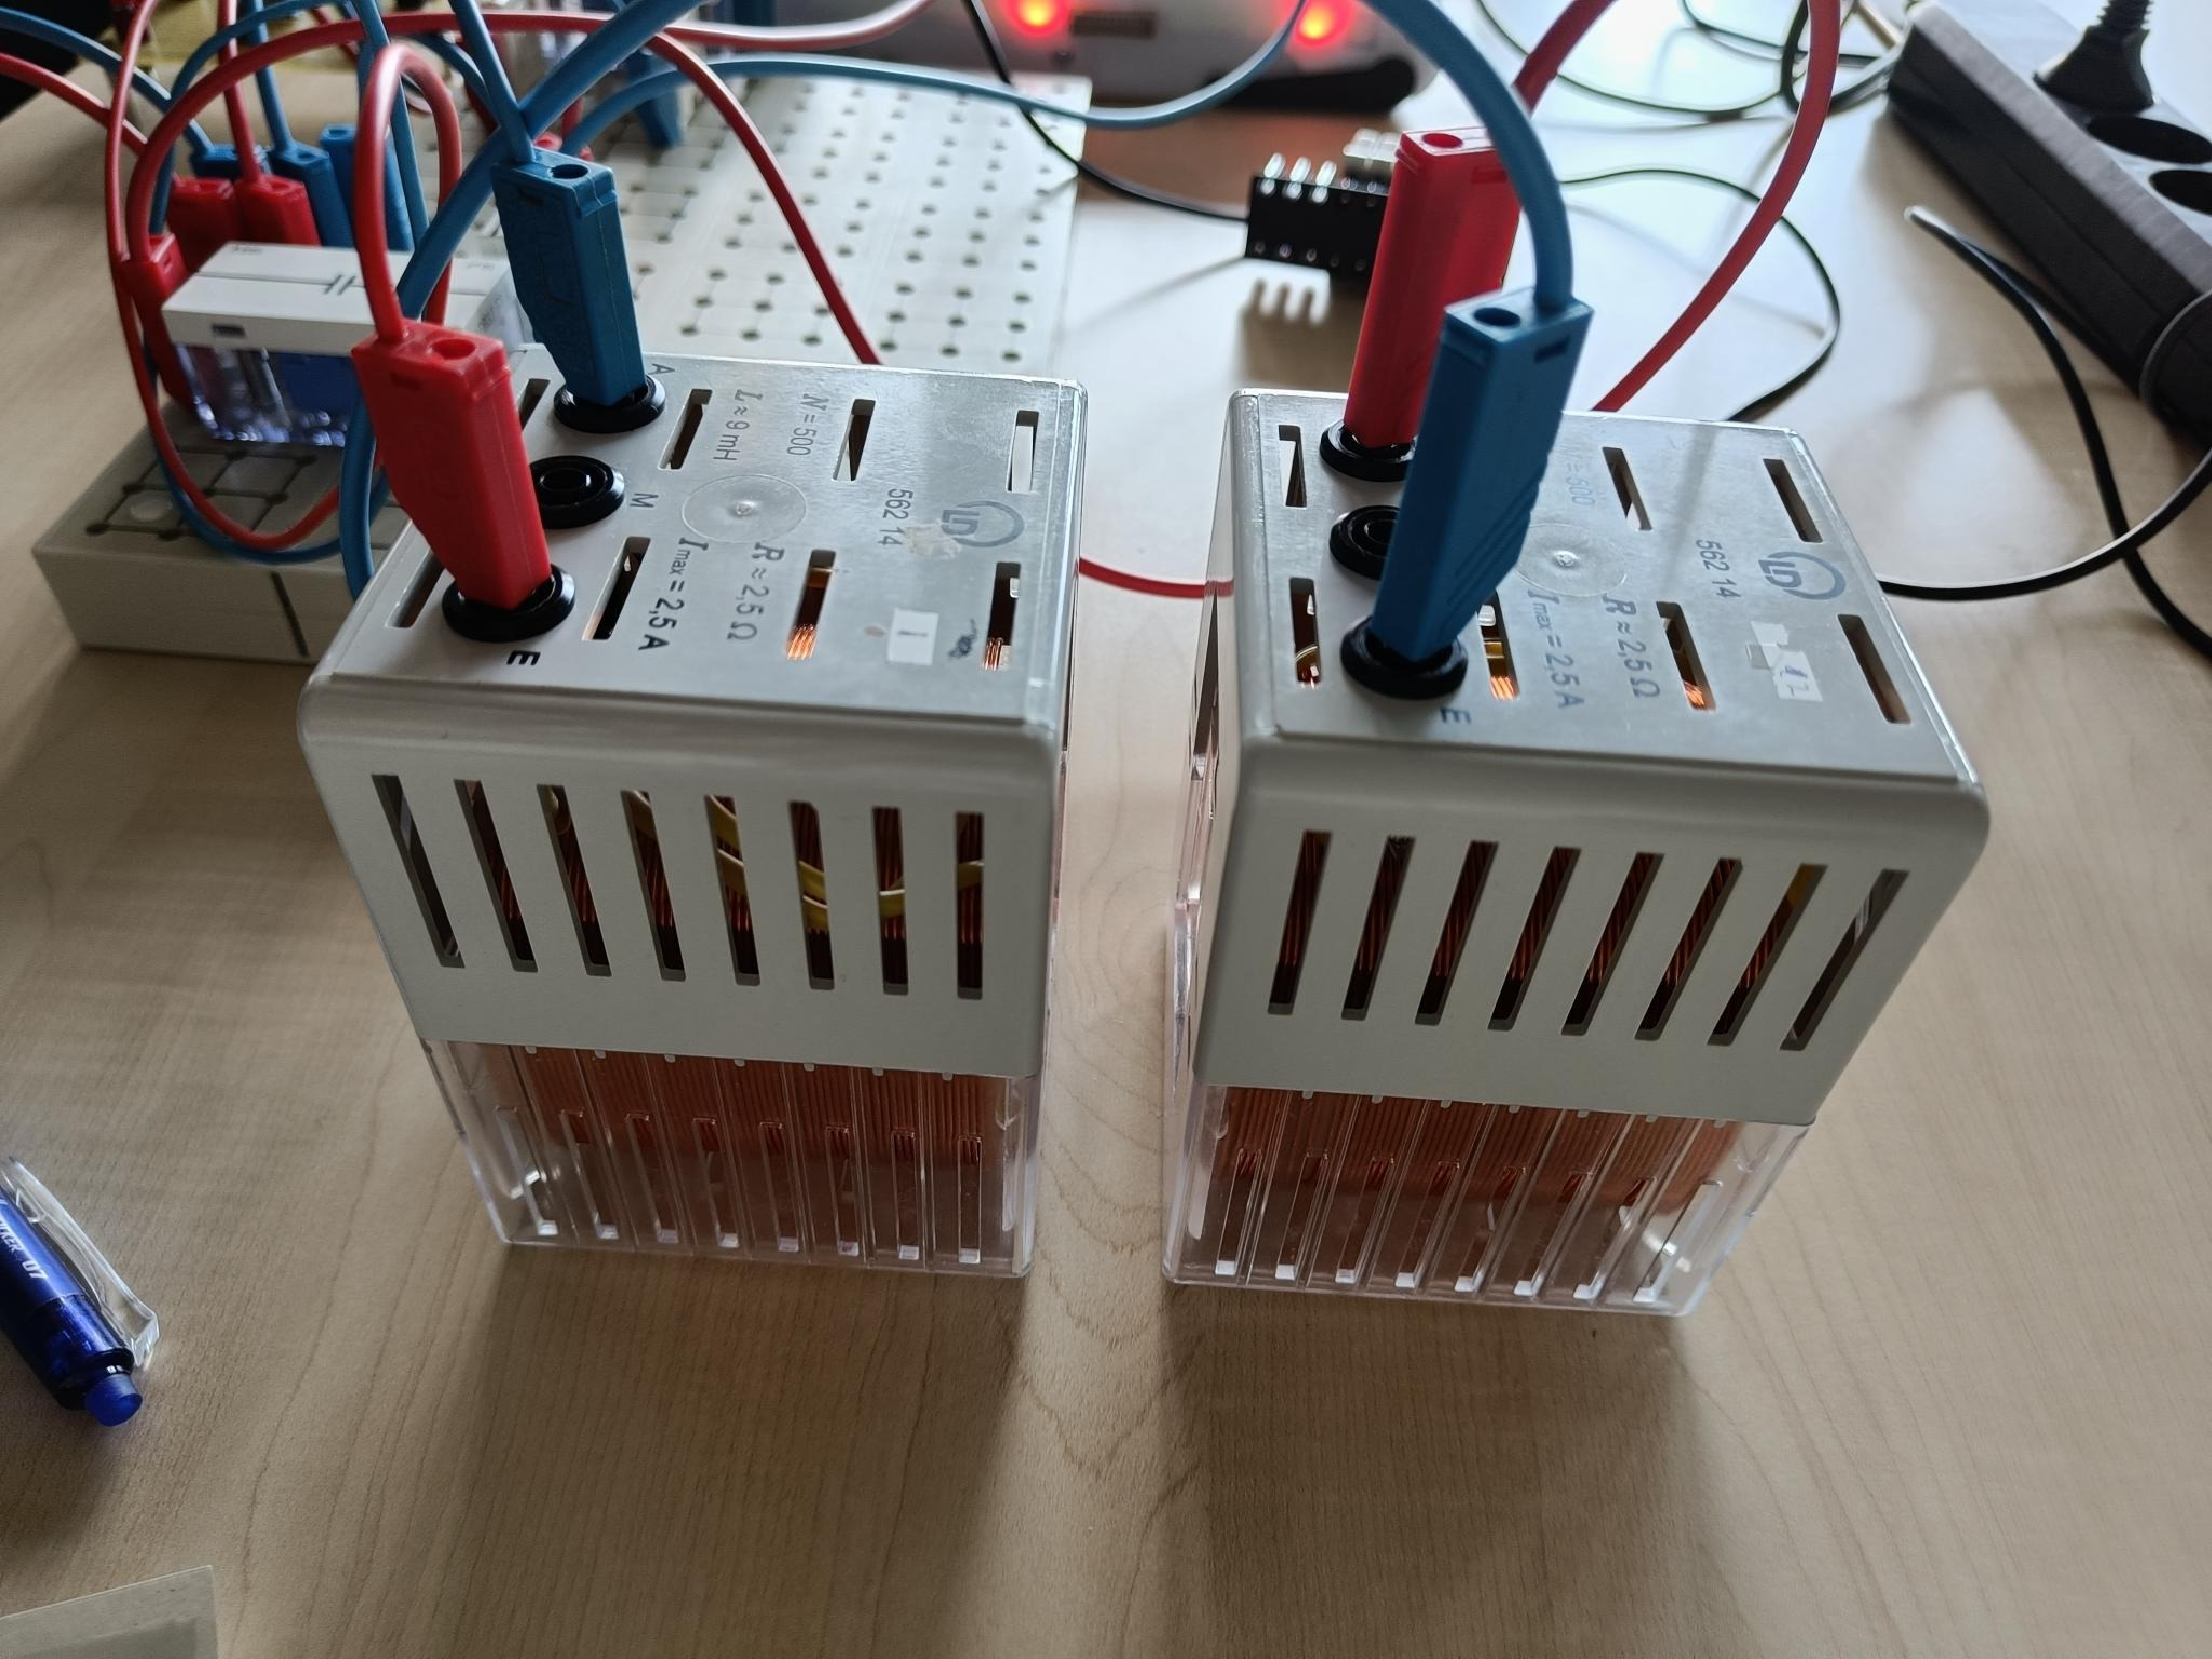
\includegraphics[width=0.8\textwidth]{bilder/Abstand_Spulen.pdf}
    \caption{Spulen im Abstand von 1cm}
\end{figure}



Dabei ist uns aufgefallen, dass in Schwingkreis 2 die zwei Fundamentalfrequenzen länger trennbar sind als im ersten. 

Zuletzt haben wir in die zwei Spulen auf einen gemeinsamen Eisenkern geschoben, um die Kopplung so zu erhöhen. Mit dieser Konfiguration haben wir die Messung noch mal durchgeführt. 

\subsubsection{Rohdaten}

Insgesamt haben wir in diesem Versuchsteil also 9 Messungen durchgeführt, 8 Messungen mit verschiedenen Abständen und eine Messung mit dem Eisenkern. 
Im Folgenden werden zu erst sämtliche Daten zu 0cm Abstand angeführt. Die Diskussion der anderen Messungen wird später durchgeführt.\\


In den unteren Grafiken, können sie den Spannungsverlauf an beiden Kondensatoren in unserem gesamten Messintervall sehen und darunter ein Ausschnitt der Schwingung. 
Hier kann man sehen, dass in dem Schwingkreis in welchem der Kondensator nicht geladen war (Schwingkreis 1) die Schwingung mit einer kleineren Amplitude startet. 
In beiden Schwingkreisen fällt die Amplitude in ca. 0.03 Sekunden auf Null ab.
Über den Genauen Verlauf der Schwingung kann diesem Graphen jedoch keine Informationen entnommen werden. 
In den Graphen in welchen wir die ersten 0.05s der Schwingung sehen, können wir sehr gut die Schwebung erkennen. 

\begin{figure}[H]
    \centering
    \includegraphics[width=0.8\textwidth]{plots/Schwebung_0cm_01_1_complete.pdf}
    \caption{Spannungsverlauf an Kondensator 1}
\end{figure}
\begin{figure}[H]
    \centering
    \includegraphics[width=0.8\textwidth]{plots/Schwebung_0cm_01_1_zoom.pdf}
    \caption{Spannungsverlauf an Kondensator 1 zoom}
\end{figure}


\begin{figure}[H]
    \centering
    \includegraphics[width=0.8\textwidth]{plots/Schwebung_0cm_01_2_complete.pdf}
    \caption{Spannungsverlauf an Kondensator 2}
\end{figure}
\begin{figure}[H]
    \centering
    \includegraphics[width=0.8\textwidth]{plots/Schwebung_0cm_01_2_zoom.pdf}
    \caption{Spannungsverlauf an Kondensator 2 zoom}
\end{figure}


Der Folgende Graph zeigt ein Zoom in des Schwingungsverlaufs von beiden Kondensatoren. Diese sind hier in einem Gemeinsamen Graphen dargestellt, dass man so die Phasenverschiebung der beiden Schwingungen gut sehen kann. 

\begin{figure}[H]
    \centering
    \includegraphics[width=1\textwidth]{plots/Schwebung_0cm_01.pdf}
    \caption{Spannungsverlauf an Kondensator 1}
\end{figure}

Hier kann man sehr gut die Phasenverschiebung zwischen den zwei Spannungen erkennen, die nach theoretischer vorhersage $\frac{\pi}{2}$ entsprechen sollte. 
Dies trifft jedoch nicht exakt zu, da wir noch einen Einfluss des Innenwiederstands der Schaltung haben.
Des weiteren ist die Periodische Modellierung der Amplitude der beiden Signale, also die Einhüllende gut zu erkennen. 
Diese hat augenscheinlich für beide Schwingkreise eine ähnliche Frequenz.
Wir können hier auch die Auswirkung des Widerstands sehen, da die Amplitude auch im Verlauf der Zeit kleiner wird. 
Dies folgt einer Exponentiellen Abnahme.

Aus der Fouriertransformation können wir die zwei Fundamentalfrequenzen des Schwingkreis bestimmen. \\

Hier ist die Komplette FFT für die Spannungsverläufe an den beiden Schwingkreisen zu sehen. Selbst ohne Zoom kann man erkennen, dass diese zwei peaks haben, hier sieht es noch so aus als würden die Peaks der zwei Schwingkreise übereinander liegen.

\begin{figure}[H]
    \centering
    \includegraphics[width=1\textwidth]{plots/Schwebung_0cm_01_FFT_complete.pdf}
    \caption{FFT der Schwingungen in Schwingkreis 1 und 2}
\end{figure}

\subsubsection{Bestimmen der Fundamentalfrequenzen}

\begin{figure}[H]
    \centering
    \includegraphics[width=1\textwidth]{plots/Schwebung_0cm_01_FFT_zoom.pdf}
    \caption{FFT-zoom der Schwingungen in Schwingkreis 1 und 2}
\end{figure}

Um die Peaks der zwei Fundamentalschwingungen zu sehen, haben wir auch einen Zoom-in der FFT betrachtet. 
Hier kann man sehr gut sehen, dass in beiden Schwingkreisen zwei Peaks vorliegen, wobei die Peaks in Schwingkreis 2 deutlich schärfer sind. 
Des weiteren kann man hier sehen, dass die Peaks leicht gegeneinander verschoben sind. Also die Fundamentalschwingungen der beiden Schwingkreise (SK) leicht voneinander abweichen werden.
Der Tiefpunkt zwischen den beiden Peaks sollte ungefähr bei der Grundfrequenz des Schwingkreises liegen.\\


Die genaue Lage der Peaks haben wir wie beim Einzelschwingkreis bestimmt, indem wir die Maxima in den entsprechenden Intervallen gesucht haben.
Hierfür haben wir aus dem Oberen Graphen den Frequenzbereich entnommen in welchem das Maximum liegen muss. So konnten wir mit einem Python Programm, jeweils die Maxima bestimmen.
Die Bestimmung der Maxima kann den zwei Graphen entnommen werden. Hier wurde das Exemplarisch für die Schwingung im SK 1 Dargestellt.

\begin{figure}[H]
    \centering
    \includegraphics[width=1\textwidth]{plots/Schwebung_0cm_01_FFT_Maximum.pdf}
    \caption{Bestimmung des Maximums von $f_+$ in SK 1}
    \label{Schwebung_Maxima}
\end{figure}


\begin{figure}[H]
    \centering
    \includegraphics[width=1\textwidth]{plots/Schwebung_0cm_01_FFT_zwei_Maximum.pdf}
    \caption{Beide Maxima in SK 1}
\end{figure}
%TODO : Messunsicherheiten auf f+ und f- 

Hier ist so wie bei den Einzelschwingkreisen einer der Fehler auf die Fundamentalfrequenz die Ableseungenauigkeit. Diese kann aus Graphik \ref{Schwebung_Maxima} entnommen werden und ist gleich zu der im Einzelschwingkreis, da wir die gleichen Messwerterfassungseinstellungen verwendet haben.
Des weiteren haben wir einen Fehler der auf Grund der statistischen Schwankung der Ergebnisse, wenn man die Messung mehrfach wiederholt. 
Diesen haben wir ebenfalls bereits bei den Einzelschwingkreisen bestimmt, indem wir SK 2 zehn mal gemessen haben. 
Hier hat sich der Statistische Fehler von $\pm 1Hz$ Ergeben.\\

Bein Sensor CASSY können wir davon ausgehen, dass wir keinen Fehler auf die Zeit haben, weswegen dies kein Einfluss auf den Fehler auf die Fundamentalfrequenzen hat.
Auf die Fundamentalfrequenzen haben wir keinen Systematischen Fehler.
Diese Fehler müssen quadratisch addiert werden, da wir davon ausgehen können, dass beide statistischer Natur sind.
So erhalten wir als Ergebnisse auf $ f_+$ und $ f_-$ in den beiden Schwingkreisen:

\begin{table}[H]
    \centering
    \begin{tabularx}{1\textwidth}{X X X X} % adjust width as needed
        \toprule
        \textbf{Schwingkreis} & \textbf{$f_+$ } & \textbf{$f_-$ } & \textbf{Fehler $(\sigma)$}\\
        \midrule
        1 & 1054Hz & 1158Hz & 1.2Hz\\
        2 & 1046Hz & 1188Hz & 1.2Hz\\
        \bottomrule
    \end{tabularx}
    \caption{Fundamentalschwingungen der zwei Schwingkreise}
    \label{•}
\end{table}

\subsubsection{Bestimmen der Eigenfrequenz und Schwebungsfrequenz}


Als weitere interessante Frequenzen, haben wir in dem gekoppelten Schwingkreis, die Frequenz der Schwebung und die Grundfrequenz des gekoppelten Schwingkreises. 
In den Grundlagen wurde bereits eingeführt wie diese mit den Fundamentalfrequenzen zusammen hängen.
Für diese ergibt sich:

\begin{equation}
    f_k = \frac{f_- + f_+}{2}
\end{equation}
\begin{equation}
    f_{schw} = \frac{f_- - f_+}{2}
\end{equation}

Für den Fehler auf diese Frequenzen müssen wir den Fehler auf $f_+$ und $f_-$ Quadratisch fortpflanzen. Aus der Gauß'schen Fehlerfortpflanzung ergibt sich:

\begin{equation}
\sigma_f =\sqrt{ \left(\frac{\partial f}{\partial f_+}\right)^2\sigma_{f_+}^2 + \left(\frac{\partial f}{\partial f_-}\right)^2\sigma_{f_-}^2}
\end{equation}

Hier steht $f$ stellvertretend für $f_k$ und $f_{schw}$. $\sigma_f$ bezeichnet die Standardabweichung auf diese Frequenzen. 
$ \sigma_{f_+} $ und $ \sigma_{f_-}$ für die Fehler auf diese Größen.

Da Jedoch der Fehler auf $f_+$ und $f_-$ gleich ist, und für die beiden Funktionen durch das quadrieren der Ableitungen das Vorzeichen keinen einfluss auf den Fehler hat ergibt sich für beide:

\begin{equation}
\sigma_f = \frac{1}{2}\sigma_{f_+}^2
\end{equation}

Mit den Fundamentalfrequenzen aus beiden Schwingkreisen ergibt sich somit:

\begin{table}[H]
    \centering
    \begin{tabularx}{1\textwidth}{X X X X} % adjust width as needed
        \toprule
        \textbf{Schwingkreis} & \textbf{$f_k$} & \textbf{$f_{schw}$} & \textbf{$\sigma_f$} \\
        \midrule
        1 & 1115Hz & 61Hz & 0.72Hz\\
        2 & 1117Hz & 71Hz & 0.72Hz \\
        \bottomrule
    \end{tabularx}
    \caption{Fundamentalschwingungen der zwei Schwingkreise}
    \label{•}
\end{table} 

\subsubsection{Bestimmung des Kopplungsgrads}

Mit den Beiden Fundamentalfrequenzen können wir ebenfalls den Kopplungsgrad bestimmen wie in den Grundlagen eingeführt.

\begin{equation}
    \Rightarrow k = \frac{f_-^2 - f_+^2}{f_-^2 + f_+^2}
\end{equation}

Hier müssen wir ebenfalls die Fehler auf $f_+$ und $f_-$ Quadratisch fortpflanzen. Wir gehen davon aus, dass diese unkorelliert sind.
\begin{equation}
\sigma_f =\sqrt{\left(\frac{4f_+f_-^2}{\left(f_+^2+f_-^2\right)^2}\sigma_{f_+}\right)^2 + \left(\frac{4f_+^2f_-}{\left(f_+^2+f_-^2\right)^2}\sigma_{f_-}\right)^2}
\end{equation}

Daraus ergibt sich für die gemessenen Frequenzen aus Schwingkreis 1 eine Kopplung von:
\begin{center}
$k_1$ = 0.094 $\pm$ 0.0015
\end{center}
und für den zweiten:
\begin{center}
$k_2$ = 0.13 $\pm$ 0.0015
\end{center}

Hier kann man sehen, dass der Kopplungsgrad den wir für Schwingkreis 1 bestimmt haben deutlich kleiner ist als der von Schwingkreis 2. 
Dies war bereits zu erwarten, da in Schwingkreis 1 die bestimmten Frequenzen deutlich enger beieinander lagen. 
%TODO : Warum ist Kopplung hier kleiner?
\subsubsection{Zeitliche Verschiebung}

Da unser Kopplungsgrad kleiner als 0.2 ist können wir als Näherung für die zeitliche Verschiebung die Formel verwenden die in den Grundlagen angegeben ist. 
Diese Zeitliche Verschiebung beschreibt, den unterschied zu unserer Erwartung von einer Phasenverschiebung von $\frac{\pi}{2}$ (zwischen Nulldurchgang der Schwebung bei Kondensator 1 und Maximum bei Kondensator 2).
  
\begin{equation}
    \Delta t \approx \frac{2 \pi}{f_{schw}} \left[ \frac{1}{\pi} - \arctan{\left( \frac{k}{R} \cdot \sqrt{\frac{L}{C}} \right)} \right]
\end{equation}

Für diese Rechnung verwenden wir den Mittelwert von $k_1$ und $k_2$ also $k = 0.112 \pm 1.06 \quad 10^{-3}$. Für L und C verwenden wir die Größen welche wir mit der Messbrücke gemessen haben und für R den Widerstand den wir aus den Einzelschwingkreisen bestimmt haben. Hier Verwende ich den Mittelwert von beiden also $ (R = \pm )\Omega $ .

\begin{aufgabe}{Gekoppelte Schwingung: gleich- und gegensinnige Anregung}
  Stellen Sie für einen festen Kopplungsgrad $k$ nacheinander die
  beiden Fundamentalschwingungen dar. Zeigen Sie jeweils die
  Fourierspektren und bestimmen Sie die zugängliche
  Eigenfrequenz. Berechnen Sie den Kopplungsgrad sowie dessen
  Messunsicherheit. Vergleichen Sie mit den Werten aus der Schwebung.
\end{aufgabe}
   
   
\end{document}

%TODO : Peak Linie aus Rohdaten raus nehmen
%TODO : Peak beschriften
